\documentclass[]{book}
\usepackage{lmodern}
\usepackage{amssymb,amsmath}
\usepackage{ifxetex,ifluatex}
\usepackage{fixltx2e} % provides \textsubscript
\ifnum 0\ifxetex 1\fi\ifluatex 1\fi=0 % if pdftex
  \usepackage[T1]{fontenc}
  \usepackage[utf8]{inputenc}
\else % if luatex or xelatex
  \ifxetex
    \usepackage{mathspec}
  \else
    \usepackage{fontspec}
  \fi
  \defaultfontfeatures{Ligatures=TeX,Scale=MatchLowercase}
\fi
% use upquote if available, for straight quotes in verbatim environments
\IfFileExists{upquote.sty}{\usepackage{upquote}}{}
% use microtype if available
\IfFileExists{microtype.sty}{%
\usepackage{microtype}
\UseMicrotypeSet[protrusion]{basicmath} % disable protrusion for tt fonts
}{}
\usepackage{hyperref}
\hypersetup{unicode=true,
            pdftitle={Bayesian Statistics for Linguists},
            pdfauthor={Masoud Jasbi},
            pdfborder={0 0 0},
            breaklinks=true}
\urlstyle{same}  % don't use monospace font for urls
\usepackage{natbib}
\bibliographystyle{apalike}
\usepackage{color}
\usepackage{fancyvrb}
\newcommand{\VerbBar}{|}
\newcommand{\VERB}{\Verb[commandchars=\\\{\}]}
\DefineVerbatimEnvironment{Highlighting}{Verbatim}{commandchars=\\\{\}}
% Add ',fontsize=\small' for more characters per line
\usepackage{framed}
\definecolor{shadecolor}{RGB}{248,248,248}
\newenvironment{Shaded}{\begin{snugshade}}{\end{snugshade}}
\newcommand{\AlertTok}[1]{\textcolor[rgb]{0.94,0.16,0.16}{#1}}
\newcommand{\AnnotationTok}[1]{\textcolor[rgb]{0.56,0.35,0.01}{\textbf{\textit{#1}}}}
\newcommand{\AttributeTok}[1]{\textcolor[rgb]{0.77,0.63,0.00}{#1}}
\newcommand{\BaseNTok}[1]{\textcolor[rgb]{0.00,0.00,0.81}{#1}}
\newcommand{\BuiltInTok}[1]{#1}
\newcommand{\CharTok}[1]{\textcolor[rgb]{0.31,0.60,0.02}{#1}}
\newcommand{\CommentTok}[1]{\textcolor[rgb]{0.56,0.35,0.01}{\textit{#1}}}
\newcommand{\CommentVarTok}[1]{\textcolor[rgb]{0.56,0.35,0.01}{\textbf{\textit{#1}}}}
\newcommand{\ConstantTok}[1]{\textcolor[rgb]{0.00,0.00,0.00}{#1}}
\newcommand{\ControlFlowTok}[1]{\textcolor[rgb]{0.13,0.29,0.53}{\textbf{#1}}}
\newcommand{\DataTypeTok}[1]{\textcolor[rgb]{0.13,0.29,0.53}{#1}}
\newcommand{\DecValTok}[1]{\textcolor[rgb]{0.00,0.00,0.81}{#1}}
\newcommand{\DocumentationTok}[1]{\textcolor[rgb]{0.56,0.35,0.01}{\textbf{\textit{#1}}}}
\newcommand{\ErrorTok}[1]{\textcolor[rgb]{0.64,0.00,0.00}{\textbf{#1}}}
\newcommand{\ExtensionTok}[1]{#1}
\newcommand{\FloatTok}[1]{\textcolor[rgb]{0.00,0.00,0.81}{#1}}
\newcommand{\FunctionTok}[1]{\textcolor[rgb]{0.00,0.00,0.00}{#1}}
\newcommand{\ImportTok}[1]{#1}
\newcommand{\InformationTok}[1]{\textcolor[rgb]{0.56,0.35,0.01}{\textbf{\textit{#1}}}}
\newcommand{\KeywordTok}[1]{\textcolor[rgb]{0.13,0.29,0.53}{\textbf{#1}}}
\newcommand{\NormalTok}[1]{#1}
\newcommand{\OperatorTok}[1]{\textcolor[rgb]{0.81,0.36,0.00}{\textbf{#1}}}
\newcommand{\OtherTok}[1]{\textcolor[rgb]{0.56,0.35,0.01}{#1}}
\newcommand{\PreprocessorTok}[1]{\textcolor[rgb]{0.56,0.35,0.01}{\textit{#1}}}
\newcommand{\RegionMarkerTok}[1]{#1}
\newcommand{\SpecialCharTok}[1]{\textcolor[rgb]{0.00,0.00,0.00}{#1}}
\newcommand{\SpecialStringTok}[1]{\textcolor[rgb]{0.31,0.60,0.02}{#1}}
\newcommand{\StringTok}[1]{\textcolor[rgb]{0.31,0.60,0.02}{#1}}
\newcommand{\VariableTok}[1]{\textcolor[rgb]{0.00,0.00,0.00}{#1}}
\newcommand{\VerbatimStringTok}[1]{\textcolor[rgb]{0.31,0.60,0.02}{#1}}
\newcommand{\WarningTok}[1]{\textcolor[rgb]{0.56,0.35,0.01}{\textbf{\textit{#1}}}}
\usepackage{longtable,booktabs}
\usepackage{graphicx,grffile}
\makeatletter
\def\maxwidth{\ifdim\Gin@nat@width>\linewidth\linewidth\else\Gin@nat@width\fi}
\def\maxheight{\ifdim\Gin@nat@height>\textheight\textheight\else\Gin@nat@height\fi}
\makeatother
% Scale images if necessary, so that they will not overflow the page
% margins by default, and it is still possible to overwrite the defaults
% using explicit options in \includegraphics[width, height, ...]{}
\setkeys{Gin}{width=\maxwidth,height=\maxheight,keepaspectratio}
\IfFileExists{parskip.sty}{%
\usepackage{parskip}
}{% else
\setlength{\parindent}{0pt}
\setlength{\parskip}{6pt plus 2pt minus 1pt}
}
\setlength{\emergencystretch}{3em}  % prevent overfull lines
\providecommand{\tightlist}{%
  \setlength{\itemsep}{0pt}\setlength{\parskip}{0pt}}
\setcounter{secnumdepth}{5}
% Redefines (sub)paragraphs to behave more like sections
\ifx\paragraph\undefined\else
\let\oldparagraph\paragraph
\renewcommand{\paragraph}[1]{\oldparagraph{#1}\mbox{}}
\fi
\ifx\subparagraph\undefined\else
\let\oldsubparagraph\subparagraph
\renewcommand{\subparagraph}[1]{\oldsubparagraph{#1}\mbox{}}
\fi

%%% Use protect on footnotes to avoid problems with footnotes in titles
\let\rmarkdownfootnote\footnote%
\def\footnote{\protect\rmarkdownfootnote}

%%% Change title format to be more compact
\usepackage{titling}

% Create subtitle command for use in maketitle
\providecommand{\subtitle}[1]{
  \posttitle{
    \begin{center}\large#1\end{center}
    }
}

\setlength{\droptitle}{-2em}

  \title{Bayesian Statistics for Linguists}
    \pretitle{\vspace{\droptitle}\centering\huge}
  \posttitle{\par}
    \author{Masoud Jasbi}
    \preauthor{\centering\large\emph}
  \postauthor{\par}
      \predate{\centering\large\emph}
  \postdate{\par}
    \date{2019-07-16}

\usepackage{booktabs}

\begin{document}
\maketitle

{
\setcounter{tocdepth}{1}
\tableofcontents
}
\hypertarget{introduction}{%
\chapter{Introduction}\label{introduction}}

\hypertarget{what-is-the-difference-between-bayesian-and-frequentist-regression}{%
\section{What is the difference between Bayesian and Frequentist regression?}\label{what-is-the-difference-between-bayesian-and-frequentist-regression}}

From MIT class by Orloff and Bloom.

Bayesian inference:

\begin{itemize}
\tightlist
\item
  uses probabilities for both hypotheses and data.
\item
  depends on the prior and likelihood of observed data.
\item
  requires one to know or construct a `subjective prior'.
\item
  dominated statistical practice before the 20th century.
\item
  may be computationally intensive due to integration over many parameters.
\end{itemize}

Frequentist inference (NHST):

\begin{itemize}
\tightlist
\item
  never uses or gives the probability of a hypothesis (no prior or posterior).
\item
  depends on the likelihood \(P(D|H)\) for both observed and unobserved data.
\item
  does not require a prior.
\item
  dominated statistical practice during the 20th century.
\item
  tends to be less computationally intensive.
\end{itemize}

\hypertarget{guidlines-for-random-effects-structure}{%
\section{Guidlines for Random Effects Structure}\label{guidlines-for-random-effects-structure}}

From Barr, et al (2013):

\begin{itemize}
\item
  If a factor is between-unit, then a random intercept is usually sufficient.
\item
  If a factor is within-unit and there are multiple observations per treatment level per unit, then you need a by-unit random slope for that factor.
\item
  The only exception to this rule is when you only have a single observation for every treatment level of every unit; in this case, the random slope variance would be completely confounded with trial-level error. It follows that a model with a random slope would be unidentifiable, and so a random intercept would be sufficient to meet the conditional independence assumption.
\end{itemize}

\hypertarget{brms}{%
\chapter{Bayesian Regression Models using BRMS}\label{brms}}

\begin{Shaded}
\begin{Highlighting}[]
\KeywordTok{library}\NormalTok{(tidyverse)}
\KeywordTok{library}\NormalTok{(lme4) }\CommentTok{# frequentist linear mixed-effects models}
\KeywordTok{library}\NormalTok{(brms) }\CommentTok{# Bayesian regression models}
\KeywordTok{library}\NormalTok{(HDInterval) }\CommentTok{# credible interval computation (highest posterier density)}
\end{Highlighting}
\end{Shaded}

\hypertarget{what-is-brms}{%
\section{What is BRMS?}\label{what-is-brms}}

BRMS is an R package for Bayesian statistical analysis developed by Paul Buerkner \citep{burkner2017brms}. It stands for Bayesian Regression Models using Stan. Stan is a probabilistic programming language developed by a team of programmers and statisticians headed by Andrew Gelman at Columbia University. It allows for developing Bayesian statistical models. BRMS provides an easy to use R interface to Stan so that instead of writing Stan code, we write our models in the familiar \texttt{lme4} langauge. BRMS translates our R code to Stan and brings back the results.

\hypertarget{continuous-dv}{%
\section{Continuous DV}\label{continuous-dv}}

Main Questions:

\begin{itemize}
\tightlist
\item
  Does voice pitch differ across female and male speakers?
\item
  How much does it depend on the social context?
\end{itemize}

We use the data provided by Franke and Roettger:

\begin{Shaded}
\begin{Highlighting}[]
\NormalTok{politedata <-}\StringTok{ }\KeywordTok{read.csv}\NormalTok{(}\StringTok{"https://raw.githubusercontent.com/michael-franke/bayes_mixed_regression_tutorial/master/code/politeness_data.csv"}\NormalTok{)}

\KeywordTok{head}\NormalTok{(politedata)}
\end{Highlighting}
\end{Shaded}

\begin{verbatim}
##   subject gender sentence context pitch
## 1      F1      F       S1     pol 213.3
## 2      F1      F       S1     inf 204.5
## 3      F1      F       S2     pol 285.1
## 4      F1      F       S2     inf 259.7
## 5      F1      F       S3     pol 203.9
## 6      F1      F       S3     inf 286.9
\end{verbatim}

Always a good idea to look at the summary of the data:

\begin{Shaded}
\begin{Highlighting}[]
\KeywordTok{summary}\NormalTok{(politedata)}
\end{Highlighting}
\end{Shaded}

\begin{verbatim}
##  subject gender sentence context      pitch      
##  F1:14   F:42   S1:12    inf:42   Min.   : 82.2  
##  F2:14   M:41   S2:12    pol:41   1st Qu.:131.6  
##  F3:14          S3:12             Median :203.9  
##  M3:14          S4:12             Mean   :193.6  
##  M4:13          S5:12             3rd Qu.:248.6  
##  M7:14          S6:11             Max.   :306.8  
##                 S7:12
\end{verbatim}

Let's plot the data:

\begin{Shaded}
\begin{Highlighting}[]
\KeywordTok{ggplot}\NormalTok{(politedata, }\KeywordTok{aes}\NormalTok{(gender, pitch, }\DataTypeTok{fill=}\NormalTok{context)) }\OperatorTok{+}\StringTok{ }
\StringTok{  }\KeywordTok{geom_boxplot}\NormalTok{() }\OperatorTok{+}\StringTok{ }\CommentTok{# create boxplots}
\StringTok{  }\KeywordTok{stat_summary}\NormalTok{(}\DataTypeTok{fun.y=}\NormalTok{mean, }
               \DataTypeTok{geom=}\StringTok{"point"}\NormalTok{, }
               \DataTypeTok{position =} \KeywordTok{position_dodge}\NormalTok{(}\DataTypeTok{width=}\FloatTok{0.75}\NormalTok{), }
               \DataTypeTok{shape=}\DecValTok{3}\NormalTok{, }
               \DataTypeTok{size=}\DecValTok{4}\NormalTok{, }
               \DataTypeTok{color=}\StringTok{"red"}\NormalTok{) }\OperatorTok{+}\StringTok{ }\CommentTok{# add the mean value to the boxplot}
\StringTok{  }\KeywordTok{geom_jitter}\NormalTok{(}\DataTypeTok{color=}\StringTok{"grey"}\NormalTok{) }\OperatorTok{+}\StringTok{ }\CommentTok{# add invidual data points with jitter so that we can see them}
\StringTok{  }\KeywordTok{theme_classic}\NormalTok{()}
\end{Highlighting}
\end{Shaded}

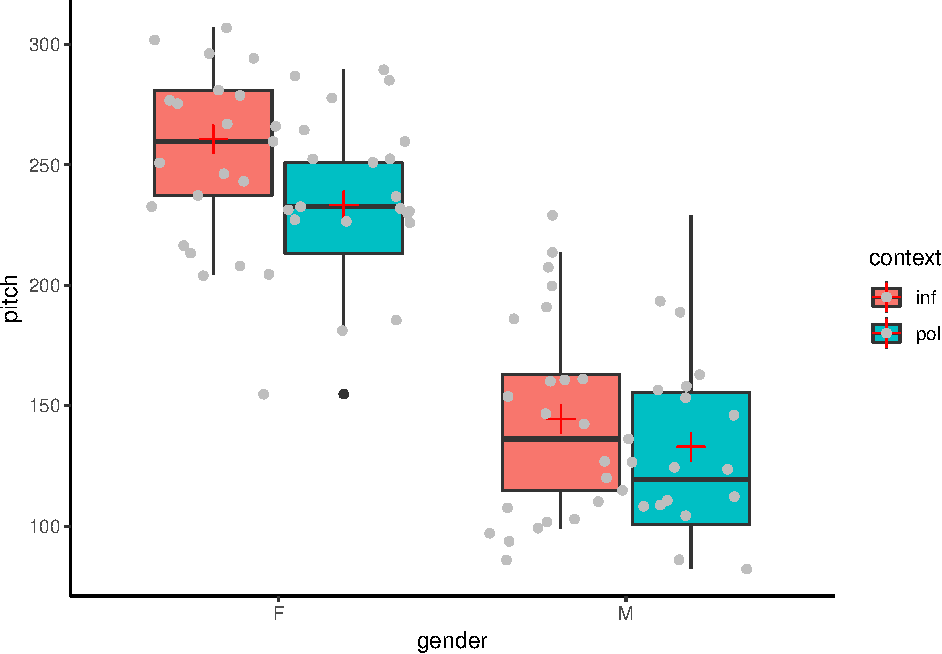
\includegraphics{mastats_files/figure-latex/politdata_plot-1.pdf}

We will consider 3 hypotheses:

\begin{itemize}
\item
  \(H_1\): Female speakers have a lower average pitch in polite than in informal contexts.
\item
  \(H_2\): Male speakers have a lower average pitch in polite than in informal contexts.
\item
  \(H_3\): Male speakers have a lower average pitch in informal than female speakers have in polite contexts.
\end{itemize}

\begin{figure}
\centering
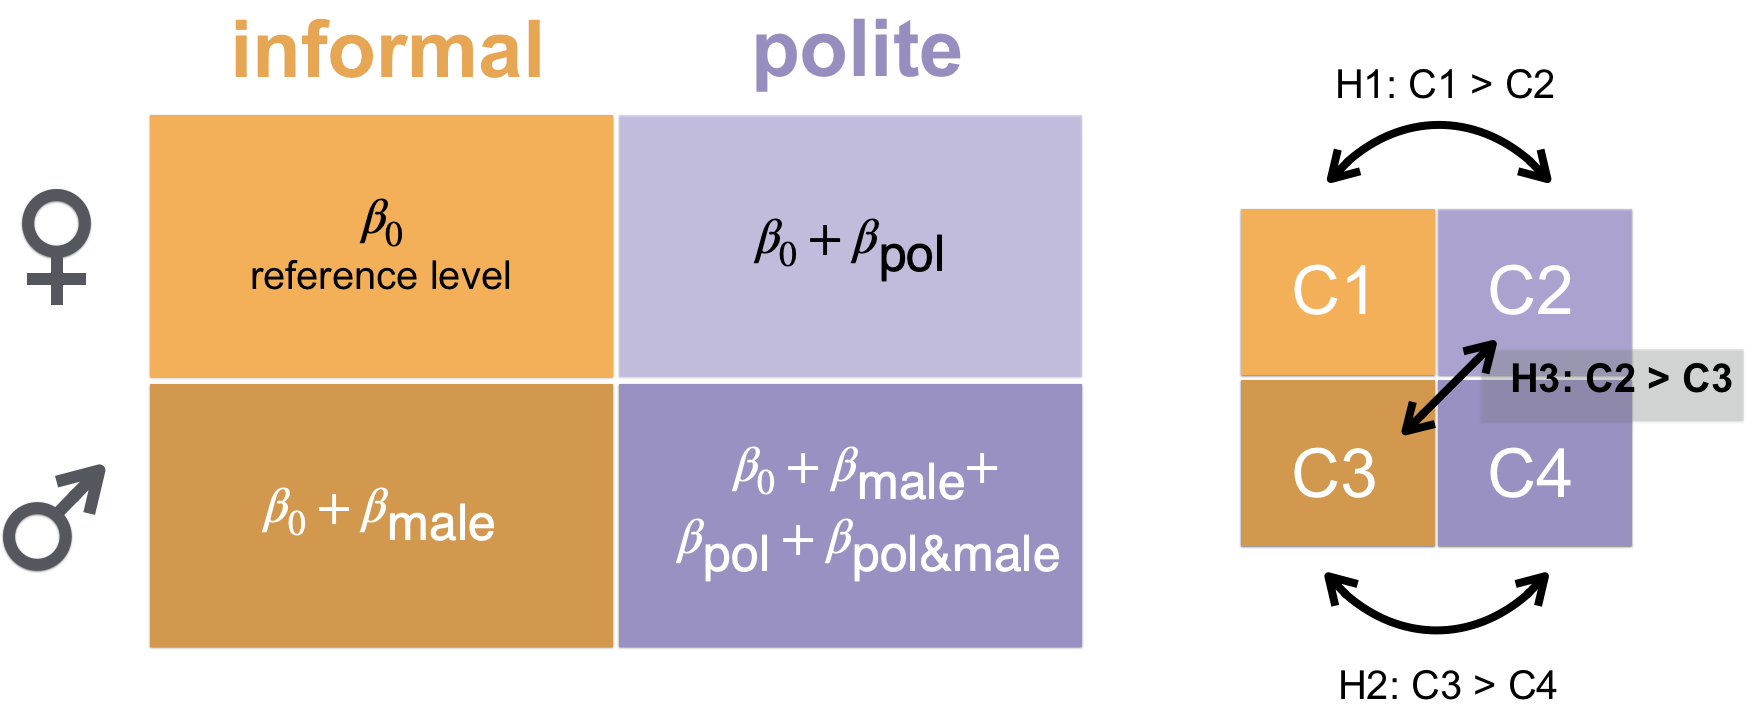
\includegraphics{pics/table_mean_hypotheses_cropped.png}
\caption{Digram of the design and the hypotheses}
\end{figure}

\hypertarget{fixed-effects-model}{%
\subsection{Fixed-effects Model}\label{fixed-effects-model}}

Let's start with a simple fixed-effects frequentist regression model using the function \texttt{lm} in R.

\begin{Shaded}
\begin{Highlighting}[]
\NormalTok{lme4Model_FE <-}\StringTok{ }\KeywordTok{lm}\NormalTok{(pitch}\OperatorTok{~}\StringTok{ }\NormalTok{gender }\OperatorTok{*}\StringTok{ }\NormalTok{context, }\DataTypeTok{data =}\NormalTok{ politedata)}

\KeywordTok{summary}\NormalTok{(lme4Model_FE)}
\end{Highlighting}
\end{Shaded}

\begin{verbatim}
## 
## Call:
## lm(formula = pitch ~ gender * context, data = politedata)
## 
## Residuals:
##     Min      1Q  Median      3Q     Max 
## -78.486 -27.383  -0.986  20.570  96.020 
## 
## Coefficients:
##                    Estimate Std. Error t value Pr(>|t|)    
## (Intercept)         260.686      7.784  33.491   <2e-16 ***
## genderM            -116.195     11.008 -10.556   <2e-16 ***
## contextpol          -27.400     11.008  -2.489   0.0149 *  
## genderM:contextpol   15.890     15.664   1.014   0.3135    
## ---
## Signif. codes:  0 '***' 0.001 '**' 0.01 '*' 0.05 '.' 0.1 ' ' 1
## 
## Residual standard error: 35.67 on 79 degrees of freedom
## Multiple R-squared:  0.7147, Adjusted R-squared:  0.7038 
## F-statistic: 65.95 on 3 and 79 DF,  p-value: < 2.2e-16
\end{verbatim}

The model shows that pitch is significantly lower for male speakers in an informal context than female speakers in an informal context. A contrast we were not interested in. The model also shows that pitch is significantly lower in a polite context than informal context for female speakers. This is our first hypothesis (\(H_1\)). Finally the model shows that there is no significant interaction between context and gender.

Let's do the same thing the Bayesian way, using \texttt{brms}:

\begin{Shaded}
\begin{Highlighting}[]
\CommentTok{# run regression model in brms}
\NormalTok{BaysModel_FE =}\StringTok{ }\KeywordTok{brm}\NormalTok{(}
  \DataTypeTok{formula =}\NormalTok{ pitch }\OperatorTok{~}\StringTok{ }\NormalTok{gender }\OperatorTok{*}\StringTok{ }\NormalTok{context,}
  \DataTypeTok{data =}\NormalTok{ politedata,}
  \DataTypeTok{family =} \StringTok{"gaussian"}\NormalTok{,}
  \DataTypeTok{file =} \StringTok{"models/BaysModel_FE"}
\NormalTok{)}

\CommentTok{# print out model_FE summary}
\NormalTok{BaysModel_FE}
\end{Highlighting}
\end{Shaded}

\begin{verbatim}
##  Family: gaussian 
##   Links: mu = identity; sigma = identity 
## Formula: pitch ~ gender * context 
##    Data: politedata (Number of observations: 83) 
## Samples: 4 chains, each with iter = 2000; warmup = 1000; thin = 1;
##          total post-warmup samples = 4000
## 
## Population-Level Effects: 
##                    Estimate Est.Error l-95% CI u-95% CI Eff.Sample Rhat
## Intercept            260.51      8.02   245.67   276.40       2358 1.00
## genderM             -116.03     11.35  -138.71   -94.06       2161 1.00
## contextpol           -27.27     11.38   -49.77    -5.01       2007 1.00
## genderM:contextpol    15.71     16.06   -15.72    47.53       1792 1.00
## 
## Family Specific Parameters: 
##       Estimate Est.Error l-95% CI u-95% CI Eff.Sample Rhat
## sigma    36.15      2.96    30.81    42.67       3329 1.00
## 
## Samples were drawn using sampling(NUTS). For each parameter, Eff.Sample 
## is a crude measure of effective sample size, and Rhat is the potential 
## scale reduction factor on split chains (at convergence, Rhat = 1).
\end{verbatim}

As you can see the results are very similar. With Bayesian models, it is important to look at the posterior distribution of our parameters, and most importantly, the trace plots of the chains to make sure they have converged.

\begin{Shaded}
\begin{Highlighting}[]
\KeywordTok{plot}\NormalTok{(BaysModel_FE)}
\end{Highlighting}
\end{Shaded}

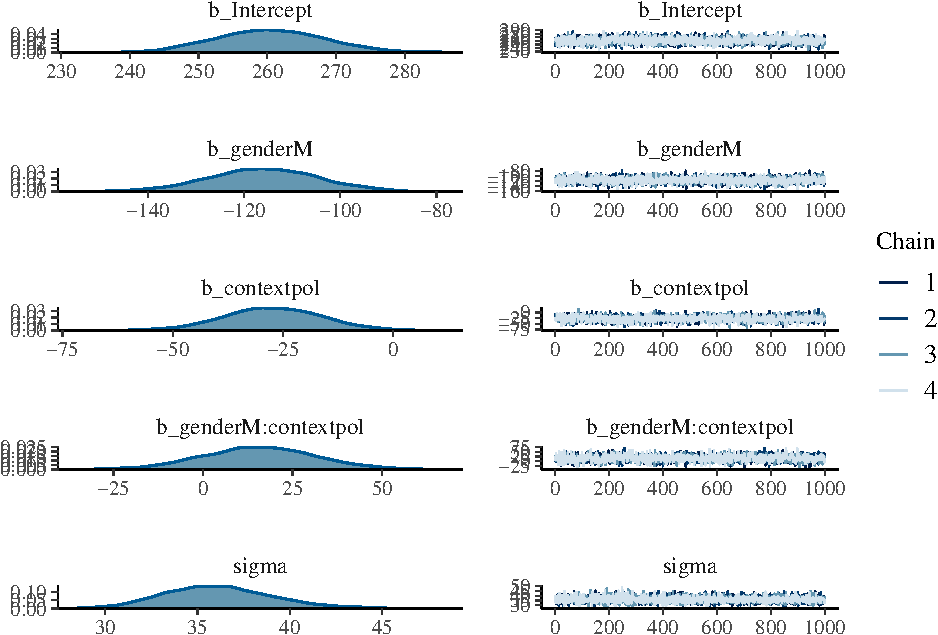
\includegraphics{mastats_files/figure-latex/tracePlots_PosteriorHistograms-1.pdf}

We can also extract the posterior samples from our model:

\begin{Shaded}
\begin{Highlighting}[]
\CommentTok{# extract posterior samples}
\NormalTok{post_samples_FE <-}\StringTok{ }\KeywordTok{posterior_samples}\NormalTok{(BaysModel_FE)}
\KeywordTok{head}\NormalTok{(post_samples_FE }\OperatorTok\StringTok{ }\KeywordTok{round}\NormalTok{(}\DecValTok{1}\NormalTok{))}
\end{Highlighting}
\end{Shaded}

\begin{verbatim}
##   b_Intercept b_genderM b_contextpol b_genderM:contextpol sigma   lp__
## 1       252.1    -110.3        -20.1                 19.5  37.0 -420.5
## 2       263.2    -119.7        -32.9                  6.7  34.4 -421.4
## 3       253.2    -104.7        -19.9                 17.2  33.7 -421.3
## 4       268.7    -120.6        -28.5                  5.5  31.4 -422.1
## 5       261.1    -116.6        -24.3                 11.9  32.7 -419.6
## 6       252.7    -123.5        -32.3                 32.2  32.9 -424.2
\end{verbatim}

Using posterior samples, we can estimate the probability of the hypotheses we are interested in. Let's consider \(H_1\): Female speakers have a lower average pitch in polite than in informal contexts. Our model estimates female pitch in the informal context as its intercept (\(\beta_0\)). It estimates female pitch in polite context as \(\beta_0 + \beta_{pol}\). Therefore, asking our model whether politeness lowers pitch in females is similar to asking if \(\beta_{pol}\) is negative (\(b_{pol} < 0\)). We are not interested in a particular sample estimate but rather, across samples, how likely is that polite context has a negative contribution? (\(P(b_{polite} < 0 | model, data)\)). We can estimate the answer using the proportion of negative samples for the politeness parameter:

\begin{Shaded}
\begin{Highlighting}[]
\KeywordTok{mean}\NormalTok{(post_samples_FE}\OperatorTok{$}\NormalTok{b_contextpol }\OperatorTok{<}\StringTok{ }\DecValTok{0}\NormalTok{)}
\end{Highlighting}
\end{Shaded}

\begin{verbatim}
## [1] 0.99225
\end{verbatim}

Now consider \(H_2\): Male speakers have a lower average pitch in polite than in informal contexts.

Consider \(H_3\): Male speakers have a lower average pitch in informal than female
speakers have in polite contexts. In our model, male pitch in informal contexts is \(\beta_{0}+ \beta_{male}\) and female pitch in polite context was \(\beta_{} + \beta_{pol}\). Therefore, hypothesis 3 boils down to: \(\beta_{pol} > \beta_{male}\)? And of course we are not interested in one particular instance of it. We want to know how likely it is that \(H_3\) is true. In other words, we are interested in \(P(\beta_{polite} > \beta_{male})\). We can estimate this probability by computing the proportion of times that this inequality holds in the posterior samples:

\begin{Shaded}
\begin{Highlighting}[]
\KeywordTok{mean}\NormalTok{(post_samples_FE}\OperatorTok{$}\NormalTok{b_contextpol }\OperatorTok{>}\StringTok{ }\NormalTok{post_samples_FE}\OperatorTok{$}\NormalTok{b_genderM)}
\end{Highlighting}
\end{Shaded}

\begin{verbatim}
## [1] 1
\end{verbatim}

Michael Franke's R package allows easy comparison between cells. First let's install and load it:

\begin{Shaded}
\begin{Highlighting}[]
\KeywordTok{library}\NormalTok{(devtools)}

\CommentTok{# install package with convenience function for Bayesian regression models for factorial designs from GitHub}
\CommentTok{#install_github(}
\CommentTok{#  repo = "michael-franke/bayes_mixed_regression_tutorial",}
\CommentTok{#  subdir = "faintr")}

\CommentTok{# load the just installed package}
\KeywordTok{library}\NormalTok{(faintr)}
\end{Highlighting}
\end{Shaded}

The function \texttt{compare\_groups} takes predictor levels and returns their mean difference, the probability of their difference being more than 0, and its credible interval.

\begin{Shaded}
\begin{Highlighting}[]
\CommentTok{# compare cell means with each other}
\KeywordTok{compare_groups}\NormalTok{(}
  \DataTypeTok{model =}\NormalTok{ BaysModel_FE,}
  \DataTypeTok{lower =} \KeywordTok{list}\NormalTok{(}\DataTypeTok{gender =} \StringTok{"M"}\NormalTok{, }\DataTypeTok{context =} \StringTok{"inf"}\NormalTok{),}
  \DataTypeTok{higher =} \KeywordTok{list}\NormalTok{(}\DataTypeTok{gender =} \StringTok{"F"}\NormalTok{, }\DataTypeTok{context =} \StringTok{"pol"}\NormalTok{)}
\NormalTok{)}
\end{Highlighting}
\end{Shaded}

\begin{verbatim}
## Outcome of comparing groups:
##  * higher:  gender:F context:pol 
##  * lower:   gender:M context:inf 
## Mean 'higher - lower':  88.76 
## 95% CI: [ 66.84 ; 110.7 ]
## P('higher - lower' > 0):  1
\end{verbatim}

\begin{Shaded}
\begin{Highlighting}[]
\NormalTok{get_posterior_beliefs_about_hypotheses =}\StringTok{ }\ControlFlowTok{function}\NormalTok{(model) \{}
  \CommentTok{# insert the comparisons you are interested in as strings }
  \KeywordTok{tibble}\NormalTok{(}
    \DataTypeTok{hypothesis =} \KeywordTok{c}\NormalTok{(}\StringTok{"Female-polite < Female-informal"}\NormalTok{, }
                   \StringTok{"Male-polite < Male-informal"}\NormalTok{,}
                   \StringTok{"Male-informal < Female-polite"}\NormalTok{),}
    \DataTypeTok{probability =} \KeywordTok{c}\NormalTok{(}
      \CommentTok{# insert the comparisons you are interested in referring to the extracted samples}
      \KeywordTok{compare_groups}\NormalTok{(}
        \DataTypeTok{model =}\NormalTok{ model, }
        \DataTypeTok{lower =} \KeywordTok{list}\NormalTok{(}\DataTypeTok{gender =} \StringTok{"F"}\NormalTok{, }\DataTypeTok{context =} \StringTok{"pol"}\NormalTok{), }
        \DataTypeTok{higher =} \KeywordTok{list}\NormalTok{(}\DataTypeTok{gender =} \StringTok{"F"}\NormalTok{, }\DataTypeTok{context =} \StringTok{"inf"}\NormalTok{)}
\NormalTok{      )}\OperatorTok{$}\NormalTok{probability,}
      \KeywordTok{compare_groups}\NormalTok{(}
        \DataTypeTok{model =}\NormalTok{ model, }
        \DataTypeTok{lower =} \KeywordTok{list}\NormalTok{(}\DataTypeTok{gender =} \StringTok{"M"}\NormalTok{, }\DataTypeTok{context =} \StringTok{"pol"}\NormalTok{), }
        \DataTypeTok{higher =} \KeywordTok{list}\NormalTok{(}\DataTypeTok{gender =} \StringTok{"M"}\NormalTok{, }\DataTypeTok{context =} \StringTok{"inf"}\NormalTok{)}
\NormalTok{      )}\OperatorTok{$}\NormalTok{probability,}
      \KeywordTok{compare_groups}\NormalTok{(}
        \DataTypeTok{model =}\NormalTok{ model, }
        \DataTypeTok{lower =} \KeywordTok{list}\NormalTok{(}\DataTypeTok{gender =} \StringTok{"M"}\NormalTok{, }\DataTypeTok{context =} \StringTok{"inf"}\NormalTok{),}
        \DataTypeTok{higher =} \KeywordTok{list}\NormalTok{(}\DataTypeTok{gender =} \StringTok{"F"}\NormalTok{, }\DataTypeTok{context =} \StringTok{"pol"}\NormalTok{)}
\NormalTok{      )}\OperatorTok{$}\NormalTok{probability }
\NormalTok{    )}
\NormalTok{  )}
\NormalTok{\}}

\KeywordTok{get_posterior_beliefs_about_hypotheses}\NormalTok{(BaysModel_FE)}
\end{Highlighting}
\end{Shaded}

\begin{verbatim}
## # A tibble: 3 x 2
##   hypothesis                      probability
##   <chr>                                 <dbl>
## 1 Female-polite < Female-informal       0.992
## 2 Male-polite < Male-informal           0.845
## 3 Male-informal < Female-polite         1
\end{verbatim}

\hypertarget{random-effects-models}{%
\subsection{Random Effects Models}\label{random-effects-models}}

\begin{Shaded}
\begin{Highlighting}[]
\NormalTok{lme4Model_RE <-}\StringTok{ }\KeywordTok{lmer}\NormalTok{(pitch }\OperatorTok{~}\StringTok{ }\NormalTok{gender}\OperatorTok{*}\NormalTok{context }\OperatorTok{+}\StringTok{ }
\StringTok{                       }\NormalTok{(}\DecValTok{1} \OperatorTok{+}\StringTok{ }\NormalTok{gender }\OperatorTok{*}\StringTok{ }\NormalTok{context }\OperatorTok{|}\StringTok{ }\NormalTok{sentence) }\OperatorTok{+}\StringTok{ }
\StringTok{                       }\NormalTok{(}\DecValTok{1} \OperatorTok{+}\StringTok{ }\NormalTok{context}\OperatorTok{|}\StringTok{ }\NormalTok{subject), }
                     \DataTypeTok{data =}\NormalTok{ politedata)}
\end{Highlighting}
\end{Shaded}

\begin{verbatim}
## boundary (singular) fit: see ?isSingular
\end{verbatim}

\begin{Shaded}
\begin{Highlighting}[]
\KeywordTok{summary}\NormalTok{(lme4Model_RE)}
\end{Highlighting}
\end{Shaded}

\begin{verbatim}
## Linear mixed model fit by REML ['lmerMod']
## Formula: pitch ~ gender * context + (1 + gender * context | sentence) +  
##     (1 + context | subject)
##    Data: politedata
## 
## REML criterion at convergence: 762.5
## 
## Scaled residuals: 
##     Min      1Q  Median      3Q     Max 
## -1.5177 -0.6585 -0.0512  0.5302  3.5188 
## 
## Random effects:
##  Groups   Name               Variance Std.Dev. Corr             
##  sentence (Intercept)        399.570  19.989                    
##           genderM            116.421  10.790   -0.97            
##           contextpol         217.655  14.753   -0.10 -0.05      
##           genderM:contextpol 293.247  17.124    0.12 -0.11 -0.78
##  subject  (Intercept)        599.757  24.490                    
##           contextpol           1.168   1.081   1.00             
##  Residual                    548.568  23.422                    
## Number of obs: 83, groups:  sentence, 7; subject, 6
## 
## Fixed effects:
##                    Estimate Std. Error t value
## (Intercept)          260.69      16.83  15.493
## genderM             -116.19      21.65  -5.367
## contextpol           -27.40       9.15  -2.994
## genderM:contextpol    15.89      12.20   1.303
## 
## Correlation of Fixed Effects:
##             (Intr) gendrM cntxtp
## genderM     -0.703              
## contextpol  -0.139  0.081       
## gndrM:cntxt  0.112 -0.142 -0.723
## convergence code: 0
## boundary (singular) fit: see ?isSingular
\end{verbatim}

\begin{Shaded}
\begin{Highlighting}[]
\KeywordTok{isSingular}\NormalTok{(lme4Model_RE)}
\end{Highlighting}
\end{Shaded}

\begin{verbatim}
## [1] TRUE
\end{verbatim}

\begin{Shaded}
\begin{Highlighting}[]
\NormalTok{BaysModel_MaxRE <-}\StringTok{ }\KeywordTok{brm}\NormalTok{(}\DataTypeTok{formula =}\NormalTok{ pitch }\OperatorTok{~}\StringTok{ }\NormalTok{gender }\OperatorTok{*}\StringTok{ }\NormalTok{context }\OperatorTok{+}
\StringTok{                    }\NormalTok{(}\DecValTok{1} \OperatorTok{+}\StringTok{ }\NormalTok{gender }\OperatorTok{*}\StringTok{ }\NormalTok{context }\OperatorTok{|}\StringTok{ }\NormalTok{sentence) }\OperatorTok{+}
\StringTok{                    }\NormalTok{(}\DecValTok{1} \OperatorTok{+}\StringTok{ }\NormalTok{context }\OperatorTok{|}\StringTok{ }\NormalTok{subject),}
                  \DataTypeTok{data =}\NormalTok{ politedata,}
                  \DataTypeTok{control =} \KeywordTok{list}\NormalTok{(}\DataTypeTok{adapt_delta =} \FloatTok{0.99}\NormalTok{),}
                  \DataTypeTok{file =} \StringTok{"models/Baysmodel_MaxRE"}\NormalTok{)}
\end{Highlighting}
\end{Shaded}

\begin{Shaded}
\begin{Highlighting}[]
\CommentTok{# Extract posterior beliefs about our hypotheses}
\KeywordTok{get_posterior_beliefs_about_hypotheses}\NormalTok{(BaysModel_MaxRE)}
\end{Highlighting}
\end{Shaded}

\begin{verbatim}
## # A tibble: 3 x 2
##   hypothesis                      probability
##   <chr>                                 <dbl>
## 1 Female-polite < Female-informal       0.981
## 2 Male-polite < Male-informal           0.816
## 3 Male-informal < Female-polite         0.990
\end{verbatim}

\begin{Shaded}
\begin{Highlighting}[]
\KeywordTok{compare_groups}\NormalTok{(}
  \DataTypeTok{model =}\NormalTok{ BaysModel_FE, }
  \DataTypeTok{lower =} \KeywordTok{list}\NormalTok{(}\DataTypeTok{gender =} \StringTok{"F"}\NormalTok{, }\DataTypeTok{context =} \StringTok{"pol"}\NormalTok{), }
  \DataTypeTok{higher =} \KeywordTok{list}\NormalTok{(}\DataTypeTok{gender =} \StringTok{"F"}\NormalTok{, }\DataTypeTok{context =} \StringTok{"inf"}\NormalTok{)}
\NormalTok{)}
\end{Highlighting}
\end{Shaded}

\begin{verbatim}
## Outcome of comparing groups:
##  * higher:  gender:F context:inf 
##  * lower:   gender:F context:pol 
## Mean 'higher - lower':  27.27 
## 95% CI: [ 4.876 ; 49.64 ]
## P('higher - lower' > 0):  0.9922
\end{verbatim}

\begin{Shaded}
\begin{Highlighting}[]
\KeywordTok{compare_groups}\NormalTok{(}
  \DataTypeTok{model =}\NormalTok{ BaysModel_MaxRE, }
  \DataTypeTok{lower =} \KeywordTok{list}\NormalTok{(}\DataTypeTok{gender =} \StringTok{"M"}\NormalTok{, }\DataTypeTok{context =} \StringTok{"pol"}\NormalTok{), }
  \DataTypeTok{higher =} \KeywordTok{list}\NormalTok{(}\DataTypeTok{gender =} \StringTok{"M"}\NormalTok{, }\DataTypeTok{context =} \StringTok{"inf"}\NormalTok{)}
\NormalTok{)}
\end{Highlighting}
\end{Shaded}

\begin{verbatim}
## Outcome of comparing groups:
##  * higher:  gender:M context:inf 
##  * lower:   gender:M context:pol 
## Mean 'higher - lower':  11.87 
## 95% CI: [ -18.05 ; 39.97 ]
## P('higher - lower' > 0):  0.8165
\end{verbatim}

\hypertarget{changing-priors}{%
\subsection{Changing Priors}\label{changing-priors}}

So far we have not explicitly provided priors for our models. \texttt{brms} has automatically assigned uninformed (uniform) priors. Let's now add some information about model priors. First let's see the priors for our fitted fixed-effects model:

\begin{Shaded}
\begin{Highlighting}[]
\KeywordTok{prior_summary}\NormalTok{(BaysModel_FE)}
\end{Highlighting}
\end{Shaded}

\begin{verbatim}
##                   prior     class               coef group resp dpar nlpar
## 1                               b                                         
## 2                               b         contextpol                      
## 3                               b            genderM                      
## 4                               b genderM:contextpol                      
## 5 student_t(3, 204, 83) Intercept                                         
## 6   student_t(3, 0, 83)     sigma                                         
##   bound
## 1      
## 2      
## 3      
## 4      
## 5      
## 6
\end{verbatim}

We can get all possible priors for our model before fitting it. Here \texttt{prior\_summary} and \texttt{get\_prior} give identical outputs because you have not specified any priors beyond the default priors:

\begin{Shaded}
\begin{Highlighting}[]
\KeywordTok{get_prior}\NormalTok{(}\DataTypeTok{formula =}\NormalTok{ pitch }\OperatorTok{~}\StringTok{ }\NormalTok{gender }\OperatorTok{*}\StringTok{ }\NormalTok{context,}
          \DataTypeTok{data =}\NormalTok{ politedata)}
\end{Highlighting}
\end{Shaded}

\begin{verbatim}
##                   prior     class               coef group resp dpar nlpar
## 1                               b                                         
## 2                               b         contextpol                      
## 3                               b            genderM                      
## 4                               b genderM:contextpol                      
## 5 student_t(3, 204, 83) Intercept                                         
## 6   student_t(3, 0, 83)     sigma                                         
##   bound
## 1      
## 2      
## 3      
## 4      
## 5      
## 6
\end{verbatim}

Let's assume that polite context does not affect pitch in female speakers. We can assign a normal prior with the mean of 0:

\begin{Shaded}
\begin{Highlighting}[]
\NormalTok{model_FE_prior =}\StringTok{ }\KeywordTok{brm}\NormalTok{(}\DataTypeTok{formula =}\NormalTok{ pitch }\OperatorTok{~}\StringTok{ }\NormalTok{gender }\OperatorTok{*}\StringTok{ }\NormalTok{context,}
                     \DataTypeTok{prior =} \KeywordTok{c}\NormalTok{(}
                       \KeywordTok{prior}\NormalTok{(}\KeywordTok{normal}\NormalTok{(}\DecValTok{0}\NormalTok{, }\DecValTok{10}\NormalTok{), }\DataTypeTok{coef =}\NormalTok{ contextpol)}
\NormalTok{                       ),}
                     \DataTypeTok{data =}\NormalTok{ politedata,}
                     \DataTypeTok{control =} \KeywordTok{list}\NormalTok{(}\DataTypeTok{adapt_delta =} \FloatTok{0.99}\NormalTok{),}
                     \DataTypeTok{file =} \StringTok{"models/model_FE_prior"}\NormalTok{)}
\end{Highlighting}
\end{Shaded}

\begin{Shaded}
\begin{Highlighting}[]
\KeywordTok{get_posterior_beliefs_about_hypotheses}\NormalTok{(model_FE_prior)}
\end{Highlighting}
\end{Shaded}

\begin{verbatim}
## # A tibble: 3 x 2
##   hypothesis                      probability
##   <chr>                                 <dbl>
## 1 Female-polite < Female-informal       0.946
## 2 Male-polite < Male-informal           0.844
## 3 Male-informal < Female-polite         1
\end{verbatim}

\begin{Shaded}
\begin{Highlighting}[]
\CommentTok{# run model without considering gender}
\NormalTok{model_FE_noGender <-}\StringTok{ }\KeywordTok{brm}\NormalTok{(}\DataTypeTok{formula =}\NormalTok{  pitch }\OperatorTok{~}\StringTok{ }\NormalTok{context,}
                        \DataTypeTok{data =}\NormalTok{ politedata,}
                        \DataTypeTok{control =} \KeywordTok{list}\NormalTok{(}\DataTypeTok{adapt_delta =} \FloatTok{0.99}\NormalTok{),}
                        \DataTypeTok{file=}\StringTok{"models/model_FE_noGender"}\NormalTok{)}
\end{Highlighting}
\end{Shaded}

\begin{Shaded}
\begin{Highlighting}[]
\CommentTok{# perform posterior predictive check fo both models}
\KeywordTok{pp_check}\NormalTok{(model_FE_noGender, }\DataTypeTok{nsample =} \DecValTok{100}\NormalTok{)}
\end{Highlighting}
\end{Shaded}

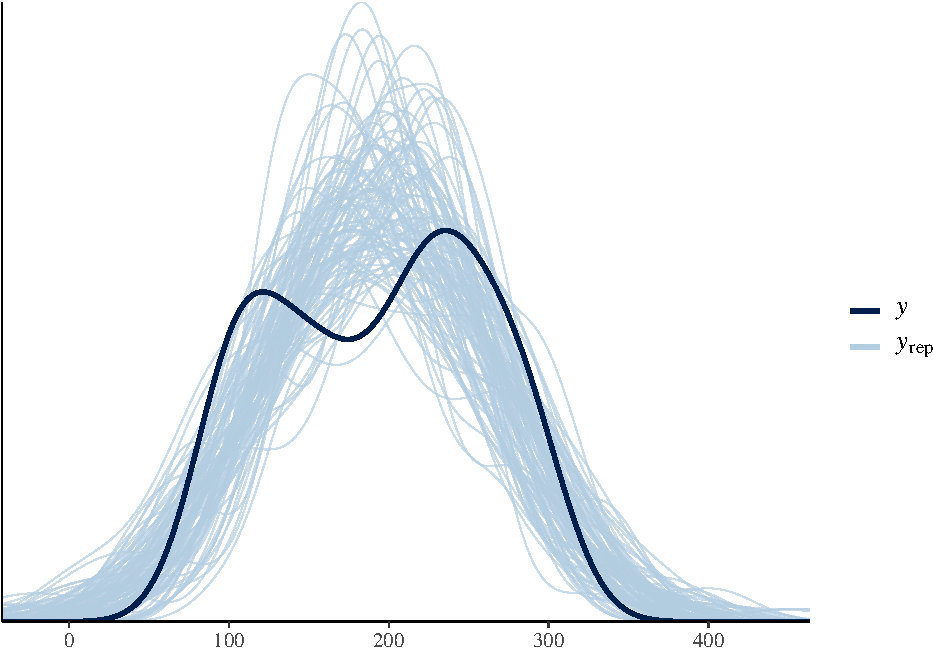
\includegraphics{mastats_files/figure-latex/unnamed-chunk-16-1.pdf}

\begin{Shaded}
\begin{Highlighting}[]
\KeywordTok{pp_check}\NormalTok{(BaysModel_FE, }\DataTypeTok{nsample =} \DecValTok{100}\NormalTok{) }
\end{Highlighting}
\end{Shaded}

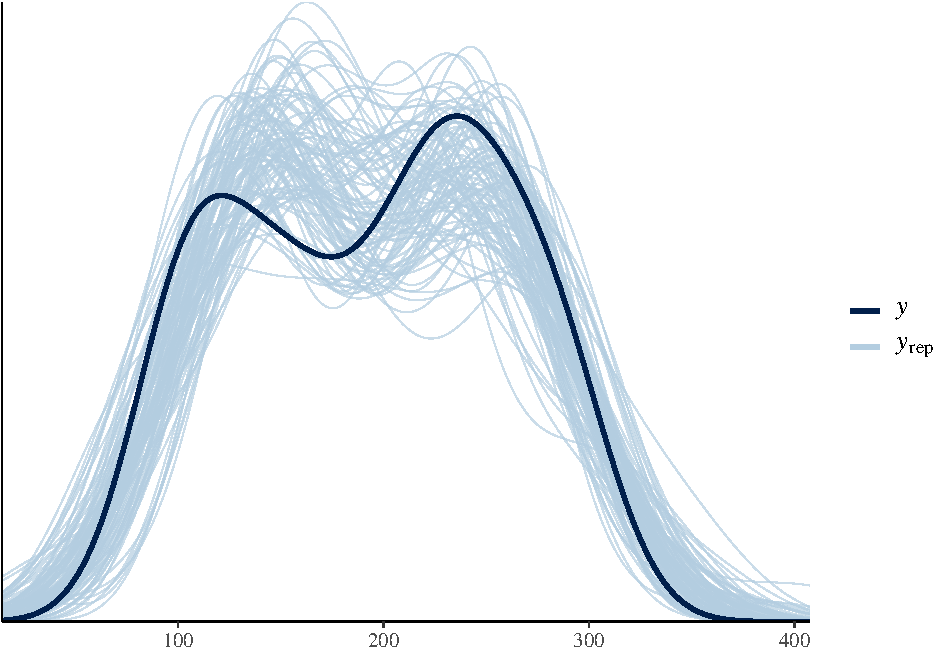
\includegraphics{mastats_files/figure-latex/unnamed-chunk-17-1.pdf}

\hypertarget{categorical-dv}{%
\section{Categorical DV}\label{categorical-dv}}

\bibliography{book.bib,packages.bib}


\end{document}
